\documentclass[preprint, 10pt]{elsarticle}

\newcommand{\mcaption}[2]{\caption{\small \em #1}\label{#2}}
\newcommand{\secref}[1]{\ref{#1}}

\usepackage{amsfonts}
\usepackage[fleqn,reqno]{amsmath}
\usepackage{amssymb}
\usepackage[titletoc]{appendix}
\usepackage{enumitem}
\usepackage{filecontents}
\usepackage[top=1.2in,bottom=1.2in,left=1in, right=1in]{geometry}
\usepackage{graphics}
\usepackage{lineno}
%\usepackage{showkeys} %To see the labels for now.  Will remove later
\usepackage{pgfplots}
\usepackage{tikz}
\usepackage{todonotes}

\usetikzlibrary{arrows}


%%%%%%  pdftex  %%%%%%%%%%%%%%%%%%%%%%%%%%%%%%%%%%%%%%%%%%%%%%%%%%%%%%
\usepackage[pagebackref=false,bookmarks=false]{hyperref} 

\hypersetup{
  bookmarksnumbered=true,
  bookmarksopen=false,
  hypertexnames=false,      
  breaklinks=true,          
  unicode=false,
  pdffitwindow=true,        
  pdfnewwindow=true,        
  colorlinks=true,         
  linkcolor=dblue,
  anchorcolor=red,
  citecolor=dorange,
  filecolor=magenta,
  urlcolor=dblue,
  pdfstartview = FitH,
  pdfkeywords = {},
  pdfcreator = {LaTeX with hyperref package}
}

\newcommand{\bd}{{\partial}}
\newcommand{\cc}{{\mathbf{c}}}
\newcommand{\DD}{{\mathcal{D}}}
\newcommand{\eeta}{{\boldsymbol\eta}}
\newcommand{\ff}{{\mathbf{f}}}
\newcommand{\grad}{{\nabla}}
\newcommand{\llambda}{{\boldsymbol\lambda}}
\newcommand{\nn}{{\mathbf{n}}}
\newcommand{\NN}{{\mathcal{N}}}
\newcommand{\pderiv}[2]{\frac{\partial #1}{\partial #2}}
\newcommand{\rr}{{\mathbf{r}}}
\newcommand{\RR}{{\mathbb{R}}}
\renewcommand{\ss}{{\mathbf{s}}}
\newcommand{\ssigma}{{\boldsymbol\sigma}}
\newcommand{\uu}{{\mathbf{u}}}
\newcommand{\UU}{{\mathbf{U}}}
\newcommand{\vv}{{\mathbf{v}}}
\newcommand{\xx}{{\mathbf{x}}}
\newcommand{\xxi}{{\boldsymbol{\xi}}}
\newcommand{\yy}{{\mathbf{y}}}


\begin{document}

\title{Methods paper for rigid bodies}

\author[Lukas]{Lukas Bystricky}
\author[Lukas]{Sachin Shanbhag}
\author[Bryan]{Bryan D.~Quaife}
\address[Lukas]{Department of Scientific Computing, Florida State University,
Tallahassee, FL, 32306.}
\address[Bryan]{Department of Scientific Computing and Geophysical Fluid
Dynamics Institute, Florida State University, Tallahassee, FL, 32306.}

\begin{abstract} 
We consider suspensions of rigid bodies in two dimensions \ldots
\end{abstract}

\begin{keyword}
  Stokes flow \sep Boundary integral method \sep Rigid body suspensions 
\end{keyword}

\maketitle





%%%%%%%%%%%%%%%%%%%%%%%%%%%%%%%%%%%%%%%%%%%%%%%%%%%%%%%%%%%%%%%%%%%%%%%
\section{Introduction\label{s:intro}}

\todo[inline]{Bryan will write this section}

This is a methods paper
\begin{itemize}
  \item Boundary integral equation formulation
  \item STIV
  \item FMM
  \item Near-singular integration
  \item Pressure and energy dissipation calculations
  \item Time integrator
\end{itemize}




%%%%%%%%%%%%%%%%%%%%%%%%%%%%%%%%%%%%%%%%%%%%%%%%%%%%%%%%%%%%%%%%%%%%%%%
\section{Formulation\label{s:formulation}} 
\subsection{Problem Formulation}

We consider a collection of rigid particles suspended in a
two-dimensional bounded or unbounded domain, $\Omega$, with boundary
$\partial\Omega$ (Figure~\ref{fig:geomSchematic}).  The boundary of the
fluid geometry is denoted by $\Gamma$ with $\Gamma_0$ being the
outermost boundary if the domain is bounded, and $\Gamma_i$, $1\leq i
\leq M_w$ are the other components of $\Gamma$.  The boundaries of rigid
particles are $\gamma_j$, $1\leq j\leq M_p$, and their union is denoted by
$\gamma$. Therefore, the boundary of the fluid domain is $ \partial\Omega
=\Gamma \cup \gamma$.
 
For each interior solid wall, we choose an interior point
$\cc^\Gamma_i$, and each rigid particle has an interior point
$\cc^\gamma_i$ and a corresponding orientation angle $\theta^\gamma_i$.
We also define the outward pointing unit normal of all these interfaces
to point out of the fluid. Finally, each solid wall has a net force and
torque, $\FF^\Gamma_i$ and $L^\Gamma_i$, respectively, that it applies
to the fluid, and similar forces and torques are defined for each rigid
body.  A schematic of the geometry is in Figure~\ref{fig:geomSchematic}.

\begin{figure}[!h]
\begin{center}
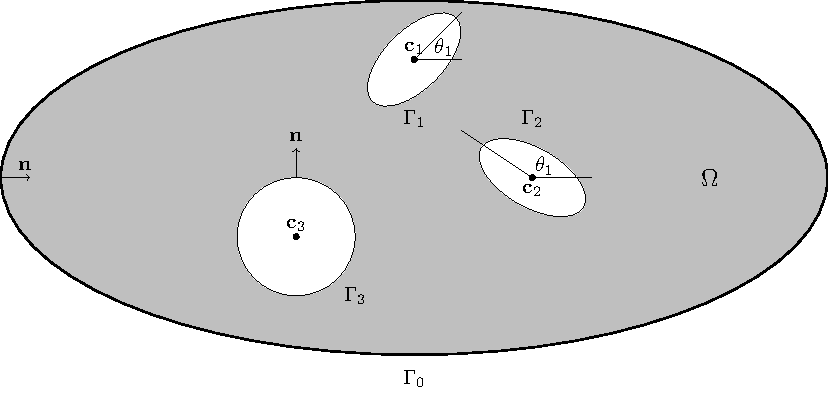
\includegraphics{figures/multiply_connected.pdf}
\end{center}
\caption{\label{fig:geomSchematic}Sketch of a fluid domain $\Omega$.
$\gamma_1$ and $\gamma_2$ enclose rigid particles, while $\Gamma_1$ is a solid
wall. The outer boundary $\Gamma_0$ may or may not be present.  The vector
$\nn$ is the unit normal vector pointing out of the fluid domain.}
\end{figure}

%%%%%%%%%%%%%%%%%%%%%%%%%%%%%%%%%%%%%%%%%%%%%%%%%%%%%%%%%%%%%%%%%%%%%%%%%%%%%%%
\subsection{Governing Equations}\label{sec:governing}
We start by assuming that the fluid is governed by the incompressible
Navier-Stokes equations 
\begin{align*}
  \rho\left(\pderiv{\uu}{t} + (\uu \cdot \grad) \uu \right) &= 
    -\grad p + \mu \Delta \uu \qquad \xx\in\Omega,\\
    \grad \cdot \uu &= 0 \qquad \xx\in\Omega,
\end{align*}
where $\uu$ is the velocity, $p$ is the pressure, $\rho$ is the fluid
density, and $\mu$ is the fluid viscosity.  The equations are
nondimensionalized in the standard method which results in the
dimensionless Reynolds number.  We are interested in small particles and
slow velocities which renders the Reynolds number small $\Re \ll 1$, and
the fluid is governed by the incompressible Stokes equations.  A
Dirichlet boundary condition $\UU$ is imposed on the solid walls
$\Gamma$, a no-slip boundary condition is assumed for the rigid bodies
$\gamma$, and the rigid bodies are assumed to be force and torque free.
\begin{equation}
  \label{eqn:modelEquations}
  \begin{split}
  \mu \Delta \uu = \grad p, &\hspace{20pt} \xx \in \Omega, \gap
    &&\mbox{\em conservation of momentum,}\\
  \grad \cdot \uu = 0, &\hspace{20pt} \xx \in \Omega, \gap
    &&\mbox{\em conservation of mass,} \\
  \uu = \UU, &\hspace{20pt} \xx \in \Gamma, \gap 
    &&\mbox{\em wall velocity,} \\
  \uu = \uu^\tau_j + \omega_j(\xx-\cc^\gamma_j)^\perp,&\hspace{20pt} 
    \xx \in \gamma, \gap &&\mbox{\em no-slip on the particles,} \\
  \FF_j^\gamma = 0, &\hspace{20pt}j=1,\ldots,M_p, \gap 
    &&\mbox{\em force-free particles,} \\
  L_j^\gamma = 0, &\hspace{20pt}j=1,\ldots,M_p, \gap 
    &&\mbox{\em torque-free particles.}
  \end{split}
\end{equation}
Here, $\uu^\tau_j$ and $\omega_j$ are the translational and rotational
velocities of rigid body $j$, respectively, and $\FF_j^\gamma$ and
$L_j^\gamma$ are the net force and torque of rigid body $j$.  For the
suspension of rigid bodies, the fluid viscosity sets the time scale, and
we assume it is one throughout the paper.  In the case of a bounded
domain, the boundary condition $\UU$ must satisfy the standard flux-free
condition, and in the case that the fluid domain is unbounded, the wall
velocity equation is replaced with a far-field condition
\begin{align*}
  \uu(\xx) = \uu_\infty(\xx), \quad |\xx| \rightarrow \infty.
\end{align*}
Then, given the rigid body translational and rotational velocities,
their centers and inclination angles $(\cc_j,\theta_j)$,
$j=1,\ldots,M_p$, satisfy
\begin{align}
\begin{split}
  \frac{d\cc_j}{dt} = \uu^\tau_j, \qquad 
  \frac{d\theta}{dt} = \omega_j.
\end{split}
\label{eqn:centersAngles}
\end{align}

While we are assuming that the rigid bodies are force-free and
torque-free, we will eventually relax this condition by allowing for a
small force and torque to guarantee that rigid bodies do not come into
unphysical contact.  This idea is first described for vesicle
suspensions by Lu et al.~\cite{Lu2017} and we summarize the method in
Section~\ref{sec:repulsion}.  

There exist many numerical methods for simulating the suspensions of
interfaces in a fluid by solving~\eqref{eqn:modelEquations} such as
level set methods, immersed boundary methods, or lattice Boltzmann
methods.  However, given that the fluid equations are linear and the
geometry mobile, we use a boundary integral equation (BIE)
formulation~\cite{Pozrikidis1992}.  BIEs have several advantages
including that only the interface has to be tracked, resulting in a
dimension reduction and simplification of complex geometries.  In the
next section we reformulate the governing
equations~\eqref{eqn:modelEquations} as a BIE.

%%%%%%%%%%%%%%%%%%%%%%%%%%%%%%%%%%%%%%%%%%%%%%%%%%%%%%%%%%%%%%%%%%%%%%%%%%%%%%%
\subsection{Boundary Integral Equation Representation}
Since the fluid equations are linear and homogeneous, a BIE formulation
is possible.  In addition to the beneficial dimension reduction, BIEs
achieve high-order accuracy, automatically satisfy the incompressibility
constraint, and can be solved with $\bigO(N)$ operations where $N$ is
the total number of points used to discretize $\bd\Omega$.  A more
detailed discussion of the BIE formulation for the incompressible Stokes
equations is discussed by Karrila and Kim~\cite{Karrila1989}.

We start by formulating the incompressible Stokes equations in the
absence of rigid bodies.  The {\em double-layer potential} is the
convolution of the stresslet with an arbitrary density
function~\cite{Ladyzhenskaya1963, Pozrikidis1992},
\begin{align}
  \label{eqn:dlp}
  \uu(\xx) = \DD[\eeta](\xx) = \frac{1}{\pi}\int_{\Gamma}
  \frac{\rr\cdot\nn}{\rho^2}\frac{\rr \otimes \rr}{\rho^2}
  \eeta(\yy)~\text{d}s_{\yy}, \quad \xx \in \Omega,
\end{align}
where $\rr = \xx - \yy$, $\rho=|\rr|$, and $\eeta$ is an unknown density
function defined on $\bd\Omega$.  The double-layer
potential~\eqref{eqn:dlp} satisfies the incompressible Stokes equations,
and a Dirichlet boundary condition $\UU$ is imposed by solving
\begin{align*}
  \lim_{\substack{\xx \rightarrow \xx_0 \\ \xx \in \Omega}}
    \DD[\eeta](\xx) = \UU(\xx_0), \quad \xx_0 \in \Gamma,
\end{align*}
for $\eeta$.  When taking the limit, the
singularity of the stresslet results in a jump~\cite{Pozrikidis1992},
and the density function must satisfy  
\begin{align}
  -\frac{1}{2} \eeta(\xx_0) + \DD[\eeta](\xx_0) = \UU(\xx_0), 
    \quad \xx_0 \in \Gamma.
  \label{eqn:secondKindBIE}
\end{align}
While the double-layer potential satisfies the incompressible Stokes
equations, it cannot represent all solutions of the incompressible
Stokes equations; in particular, it cannot represent rigid body motion.
This is rectified by introducing point forces and torques due to each
interior component of the geometry $\Gamma_j$~\cite{Power1987,
Power1993}.  To accomplish this we introduce the velocity fields due to a
point force $\mathbf{S}(\xx,\cc)$ (Stokeslet) and due to a 
point torque $\mathbf{R}(\xx,\cc)$ (rotlet) both centered at $\cc$,
\begin{align*}
  \mathbf{S}(\xx,\cc) = -\log\rho\mathbf{I} + 
  \frac{\rr \otimes \rr}{\rho^2}, \quad \text{and} \quad
  \mathbf{R}(\xx,\cc) = \frac{\rr^\perp}{\rho^2},
\end{align*}
where $\rr = \xx - \cc$ and $\rho = |\rr|$.  Then, the second-kind
integral equation~\eqref{eqn:secondKindBIE} is replaced with the
completed second-kind BIE
\begin{equation}
  \label{eqn:completed_DLP}
  \begin{split}
  -\frac{1}{2}\eeta(\xx_0) + \DD[\eeta](\xx_0) + 
    \sum_{j=1}^{M_w} \left(\mathbf{S}(\xx,\cc^\Gamma_j)\FF^\Gamma_j + 
      \mathbf{R}(\xx,\cc^\Gamma_j)L^\Gamma_j\right) &= \UU(\xx_0),
      \quad &&\xx_0 \in \Gamma, \\
  \int_{\Gamma_j} \eeta~\text{d}s &= \FF^\Gamma_j, 
      &&j=1,\ldots,M_w, \\
  \int_{\Gamma_j} \eeta\cdot (\xx - \cc^\Gamma_j)^\perp~\text{d}s &=   
      L^\Gamma_j, &&j=1,\ldots,M_w.
  \end{split}
\end{equation}
The closure formula relating the strength of the Stokeslets and rotlets
guarantees the existence of a density function, Stokeslets, and rotlets
given an admissible boundary condition $\UU$.  This is the method of
Power and Miranda~\cite{Power1987} and Power~\cite{Power1993} to
relate the density function on the rigid bodies to the corresponding
force and torque.

We now introduce a suspension of rigid bodies $\gamma_j$,
$j=1,\ldots,M_p$.  Imposing the no-slip boundary condition on the rigid
bodies, the BIE formulation of the suspension of rigid bodies governed
by equation~\eqref{eqn:modelEquations} is
\begin{subequations}
  \label{eqn:BIEformulation}
  \begin{align}
    \UU(\xx) &= -\frac{1}{2}\eeta(\xx) + \DD[\eeta](\xx) +
    \sum_{j=1}^{M_w} \left(\mathbf{S}(\xx,\cc^\Gamma_j)\FF^\Gamma_j + 
      \mathbf{R}(\xx,\cc^\Gamma_j)L^\Gamma_j\right)  \nonumber \\
&\hspace{96pt}+\sum_{j=1}^{M_p} \left(\mathbf{S}(\xx,\cc^\gamma_j)\FF^\gamma_j +
\mathbf{R}(\xx,\cc^\gamma_j)L^\gamma_j\right),
    \quad \xx \in \Gamma, \label{eqn:BIEformulation1} \\
  \uu^\tau_j + \omega_j(\xx - \cc_j^\gamma)^\perp &=
    -\frac{1}{2}\eeta(\xx) + \DD[\eeta](\xx) + 
    \sum_{j=1}^{M_w} \left(\mathbf{S}(\xx,\cc^\Gamma_j)\FF^\Gamma_j + 
      \mathbf{R}(\xx,\cc^\Gamma_j)L^\Gamma_j\right) \nonumber \\
&\hspace{96pt}+\sum_{j=1}^{M_p} \left(\mathbf{S}(\xx,\cc^\gamma_j)\FF^\gamma_j +
\mathbf{R}(\xx,\cc^\gamma_j)L^\gamma_j\right),
    \quad \xx \in \gamma, \label{eqn:BIEformulation2} \\
  \int_{\Gamma_j} \eeta~\text{d}s &= \FF^\Gamma_j, \quad
  \int_{\Gamma_j} \eeta\cdot (\xx - \cc^\Gamma_j)^\perp~\text{d}s =
  L^\Gamma_j, \quad j=1,\ldots,M_w, \label{eqn:BIEformulation3} \\
  \int_{\gamma_j} \eeta~\text{d}s &= \FF^\gamma_j, \quad
  \int_{\gamma_j} \eeta\cdot (\xx - \cc^\gamma_j)^\perp~\text{d}s =
  L^\gamma_j,\quad j=1,\ldots,M_p, \label{eqn:BIEformulation4} \\
  \FF^\gamma_j &= 0, \quad \L^\gamma_j = 0,\quad j=1,\ldots,M_p.
  \label{eqn:BIEformulation5}
\end{align}
\end{subequations}
Again, we have used the methodology of Power and
Miranda~\cite{Power1987, Power1993} to relate the strength of the Stokeslets and
rotlets of each rigid body to its density function. The reformulation
of the governing equations in Equation~\eqref{eqn:BIEformulation}
constitutes eight equations for eight unknowns: the density function,
net force, and net torque on the solid walls and rigid bodies, and the
translational and rotational velocities.  

While~\eqref{eqn:BIEformulation1} and~\eqref{eqn:BIEformulation2} are
both numerically desirable second-kind Fredholm integral equations
equations, equation~\eqref{eqn:BIEformulation1} has a rank one null
space because of the flux-free condition of the boundary data
$\UU$~\cite{Ladyzhenskaya1963}.  Following~\cite{Power1993}, this null
space is removed by adding the term 
\begin{align}
\label{eqn:N0_modification} 
  \mathcal{N}_0[\eeta](\xx) = \int_{\Gamma_0} 
    \nn(\xx)\otimes\nn(\yy)~\text{d}s(\yy)
\end{align}
to~\eqref{eqn:BIEformulation1}, but only for points $\xx \in \Gamma_0$.
Finally, if $\Omega$ is unbounded, there is no null space, and
the only modification to~\eqref{eqn:BIEformulation} is that
equation~\eqref{eqn:BIEformulation1} is removed and
equation~\eqref{eqn:BIEformulation2} has the background velocity
$\uu_\infty(\xx)$ added to the right hand side.


%%%%%%%%%%%%%%%%%%%%%%%%%%%%%%%%%%%%%%%%%%%%%%%%%%%%%%%%%%%%%%%%%%%%%%%%%%%%%%%
\subsection{A contact based repulsion force}
\label{sec:repulsion}
Exact solutions of the Stokes equations prohibit contact between
force-free and torque-free particles in finite time.  Therefore, any
contact between rigid bodies is caused by numerical errors.  The two main sources of error are
the quadrature error---especially for nearly touching rigid bodies---and
time stepping error.  Issues with quadrature have been addressed using
near-singular integration techniques~\cite{Ying2006, Klockner2013,
Quaife2014, Barnett2015, Beale2001, Cortez2001},
and high-order or even spectral accuracy in space can be achieved.
Errors due to time stepping have recently received more attention, and
methods that control stiffness~\cite{Quaife2014}, and use adaptive time step sizes~\cite{Kropinski1999,
Quaife2015, Sorgentone2018}.

%When evaluating a target point close to the boundary (as is
%necessary when two particles come close together) the kernel in the
%double layer potential becomes very sharply peaked and thus difficult to
%integrate accurately. Spatial and temporal adaptivity
%\cite{Kropinski1999}, special integration techniques \cite{Klockner2013,
%Ying2006} or asymptotic expansions of lubrication forces
%\cite{Mammoli2006} are all tools that can help, however even if we
%evaluate the double layer potential accurately, time stepping errors can
%still lead to contact. To keep computational costs reasonable we must
%turn to alternative approaches. 

%\begin{figure}[!h]\label{fig:collision_sketch}
%\begin{center}
%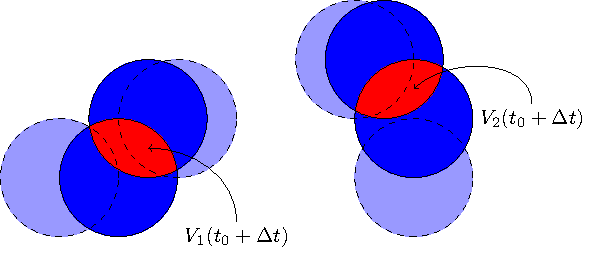
\includegraphics{figures/collisions.pdf}
%\end{center}
%\caption{Sketch of potential collisions.}
%\end{figure}

 Alternatively, repulsion forces can be added~\cite{Malhotra2018}, or
the analytic solutions of the flow due to lubrication forces can be
added to the dynamics~\cite{Mammoli2006}.  Unfortunately, repulsion
forces often introduce non-linear stiffness that restricts the time step
size, and using lubrication theory is difficult for particles of arbitrary
geometry due to the complicated asymptotics needed.

We adopt the method of introducing an artificial force to avoid
collision. There are many possible choices for the type of force. One
possibility is a repulsion force based on a Morse or Lennard-Jones type
potential that grows as a high order polynomial as two particles become
close together~\cite{Flormann2017, Liu2006}. This has been shown to work
for dense suspensions, however the resulting ODEs become very stiff as
the separation between particles decreases, thus requiring smaller time
steps. Spring based models~\cite{Tsubota2006, Zhao2013, Kabacogulu2017}
have also been used to generate artificial repulsion forces, although
these models also introduce stiffness. One further disadvantage of these
methods is that neither approach explicitly guarantees no contact
between particles. If too large a time step is chosen collisions can
still occur. 


Our approach mirrors~\cite{Lu2017} where the choice of forces and
torques guarantee that each time step is collision-free.
It is well known that the Stokes equations are the Euler-Lagrange
for a variational problem,
\begin{align*}
  \min \int_{\Omega} \nabla\uu:\nabla\uu~\text{d}\Omega,
  \quad\text{ such that }\quad \nabla\cdot\uu = 0 \text{ in }\Omega.
\end{align*} 
In the Euler-Lagrange equations, the pressure $p$ is the Lagrange
multiplier associated with the incompressibility constraint. In \cite{Lu2017}, an
additional constraint that requires the configuration of rigid particles
to be contact-free is imposed. This constraint necessitates an
additional Lagrange multiplier $\lambda$ which determines the magnitude
of the repulsion force. The direction comes from the response of the
contact volume to changes in the velocity. To solve for $\lambda$
requires the solution of a nonlinear complementary problem (NCP). This
NCP can be linearized, leading to a sequence of linear complementary
problems that must be solved at each time step.




%%%%%%%%%%%%%%%%%%%%%%%%%%%%%%%%%%%%%%%%%%%%%%%%%%%%%%%%%%%%%%%%%%%%%%%%%%%%%%%
%\begin{comment}
%\subsection{Avoiding Contact with STIV}
%Before discussing how collisions can be resolved, we first define a
%metric that measures collision.  This metric should track all pairwise
%collisions and detect if a two particles overlapped not only at the
%discrete time points, but at any time.  We let $\mathbf{V}(t)$ be a
%vector with size $\binom{M_p}{2}$ which is the total number of possible
%pairwise collisions.  $\mathbf{V}$ should be defined in such a way that
%it is 0 if no collisions have occurred, and if there is a collision, its
%value should quantify the amount of overlap.   Then, if there is a
%collision between two particles, the repulsion force should be chosen to
%scale with the magnitude of the corresponding entry of $\mathbf{V}$.
%There are several possible choices for $\mathbf{V}(t)$, the simplest
%being a signed distance between all points on all particles. We use the
%concept of {\em Space-Time Interference Volumes} (STIV) introduced by
%Harmon et al.~\cite{Harmon2011} and adapted for the suspension of
%deformable and rigid particles~\cite{Lu2017}. STIVs involve a time
%integral and are therefore more expensive to compute than other metrics
%(e.g. a signed distance). In most simulations however the cost of
%computing an STIV is dwarfed by the cost of the linear solves necessary
%to compute the velocities of the particles. The advantage of STIVs
%compared to simpler metrics is that under the assumption of ballistic
%motion they are able to detect collisions between two particles that
%pass completely through one another, i.e. it can detect that a collision
%has occurred even if the final candidate configuration is contact-free.
%
%%%%%%%%%%%%%%%%%%%%%%%%%%%%%%%%%%%%%%%%%%%%%%%%%%%%%%%%%%%%%%%%%%%%%%%%%%%%%%%%%\subsection{Variational Formulation}
%The incompressible Stokes equations can be can be restated as a minimization
%problem. Consider the functional,
%\[ \mathcal{J}(\mathbf{u}) = \int_{\Omega} \nabla\mathbf{u}:\nabla\mathbf{u} -
%2\mathbf{f}\cdot\mathbf{u} ~\text{d}\Omega,\]
%and the associated constrained minimization problem,
%\[ \min \mathcal{J}(\mathbf{u}) ~:~ \nabla\cdot\mathbf{u} = 0 \text{ in
%}\Omega.\]
%Introducing $p$, a Lagrange multiplier for the incompressibility condition, we
%can construct a Lagrangian for this system,
%\begin{equation}\label{eq:lagrangian} \mathcal{L}(\mathbf{u},p) =
%\mathcal{J}(\mathbf{u}) - \int_{\Omega}
%2p\nabla\cdot\mathbf{u}~\text{d}\Omega.\end{equation}
%First order optimality (KKT) conditions for $\mathcal{L}(\mathbf{u},p)$
%recover the incompressible Stokes equations. For our problem, in
%addition to the incompressibility condition, we wish to enforce the
%constraint that the solution $\mathbf{u}$ at a time $t_0$ should not
%introduce collisions at time $t_0+\Delta t$, in other words
%$\mathbf{V}(t_0 + \Delta t) \geq \mathbf{0}$.  This constraint can be
%incorporated in the Lagrangian \eqref{eq:lagrangian} with the
%introduction of a Lagrange multiplier $\llambda$ with one component
%for each possible collision volume,
%\begin{equation}\label{eq:lagrangian2} \tilde{\mathcal{L}}(\mathbf{u},p,\lambda)= \mathcal{L}(\mathbf{u},p) + \pmb{\lambda} \cdot \mathbf{V}(t_0+\Delta
%t).\end{equation}
%First order optimality for \eqref{eq:lagrangian2} yields the Stokes equations
%with a modified forcing function,
%\begin{equation}\label{eq:stokes_mod}-\Delta \mathbf{u} + \nabla p = \mathbf{f}%+ \int_{\Omega} \text{d}_{\mathbf{u}} \mathbf{V}^T\pmb{\lambda}
%~\text{d}\Omega,\end{equation}
%subject to the constraints
%\[ \nabla\cdot\mathbf{u} =0, ~\mathbf{V}(t_0 + \Delta t) \geq 0,~\pmb{\lambda}
%\geq 0, ~ \pmb{\lambda}\cdot\mathbf{V}(t_0+\Delta t) = 0. \]
%
%The constraints on $\mathbf{V}$ and $\pmb{\lambda}$ can be combined into a
%single constraint,
%\begin{equation}\label{eq:ncp_constraint} \mathbf{V}(t_0 + \Delta t)\geq
%\mathbf{0} \perp \pmb{\lambda}\geq \mathbf{0}.\end{equation}
%
%\end{comment}
%%%%%%%%%%%%%%%%%%%%%%%%%%%%%%%%%%%%%%%%%%%%%%%%%%%%%%%%%%%%%%%%%%%%%%%%%%%%%%%


%%%%%%%%%%%%%%%%%%%%%%%%%%%%%%%%%%%%%%%%%%%%%%%%%%%%%%%%%%%%%%%%%%%%%%%%%%%%%%%
\begin{comment}
\subsection{Complementary Problem}

To compute the repulsion forces we must first compute $\pmb{\lambda}$ for each
time step such that \eqref{eq:ncp_constraint} is satisfied.
Consider particles suspended in a fluid in an ambient flow $\mathbf{u}_\infty$.
This flow can be an imposed background flow or come from solid walls. In the
later case this velocity field is computed by solving the appropriate resistance problem. In either case this flow can be expressed as the sum of a translational component $\mathbf{u}_{\infty}^\tau$, a rotational component $\omega_{\infty}$
and a strain component $\mathbf{e}_{\infty}$,
\[ \mathbf{u}_{\infty}(\mathbf{x}) = \mathbf{u}_{\infty}^\tau +
\omega_\infty\times \mathbf{x} + \mathbf{e}_\infty \cdot\mathbf{x}.\]
The translational and rotational velocity as well as the density
function of a collection of particles can be computed from the force,
torque and strain rate~\cite{Karrila1991},
\begin{equation}\label{eq:mobility} \begin{bmatrix} \mathbf{u}_\infty^\tau -
\mathbf{u}_\tau\\ \omega^\infty - \omega \\\pmb{\eta}\end{bmatrix} =
\mathcal{M}\begin{bmatrix}\mathbf{F}\\\mathbf{L}\\\mathbf{e}_\infty\end{bmatrix},\end{equation}
where $\mathcal{M}$ is the {\em mobility tensor} and depends only on the
particle configuration $\mathbf{q}^0$ at some time $t^0$. Assuming the
only force and torques acting on particles arises from repulsion forces,
we can decompose \eqref{eq:mobility} as,
\[ \begin{bmatrix} \mathbf{u}_\infty^\tau - \mathbf{u}_\tau\\ \omega^\infty -
\omega \\\pmb{\eta}\end{bmatrix} =
\mathcal{M}\begin{bmatrix}\mathbf{0}\\\mathbf{0}\\\mathbf{e}_\infty\end{bmatrix}+
\mathcal{M}\begin{bmatrix}\mathbf{F}_c\\\mathbf{L}_c\\\mathbf{0}\end{bmatrix}.\]Once
we solve for $\mathbf{u}_\tau$ and $\omega$ we can update the positions an
dangles of each particle using an explicit Euler step. With an abuse of
notation,
this lets us express a candidate configuration $\mathbf{q}^{1}$ as,
\[ \mathbf{q}^{1} = \mathbf{q}^n + \Delta
t\left(\mathcal{M}\begin{bmatrix}\mathbf{0}\\\mathbf{0}\\\mathbf{e}_\infty\end{bmatrix}
+
\mathcal{M}\begin{bmatrix}\mathbf{F}_c\\\mathbf{L}_c\\\mathbf{0}\end{bmatrix}\right).\]

This candidate configuration must satisfy the constraint
\eqref{eq:ncp_constraint}, which we will rewrite to show the dependence of
$\mathbf{V}$ on both $\mathbf{q}^0$ and $\mathbf{q}^{1}$,
\begin{equation}\label{eq:ncp_new}\mathbf{V}(\mathbf{q}^0,\mathbf{q}^{1})\geq
\mathbf{0}\perp \pmb{\lambda}^n\geq \mathbf{0} \Rightarrow
\mathbf{V}\left(\mathbf{q}^0, \mathbf{q}^0 + \Delta
t\left(\mathcal{M}\begin{bmatrix}\mathbf{0}\\\mathbf{0}\\\mathbf{e}_\infty\end{bmatrix}
+
\mathcal{M}\begin{bmatrix}\mathbf{F}_c\\\mathbf{L}_c\\\mathbf{0}\end{bmatrix}\right)\right)
\geq \mathbf{0} \perp\pmb{\lambda}\geq \mathbf{0} .\end{equation}

This is a nonlinear complementary problem (NCP). We can see this by explicitly
including the dependence of $\mathbf{V}$ on $\pmb{\lambda}$,
\[\mathbf{V}\left(\mathbf{q}^0, \mathbf{q}^0 + \Delta
t\left(\mathcal{M}\begin{bmatrix}\mathbf{0}\\\mathbf{0}\\\mathbf{e}_\infty\end{bmatrix}
+ \mathcal{M}\begin{bmatrix} \int_{\Gamma_k}
\text{d}_\mathbf{u}\mathbf{V}^T\pmb{\lambda}~\text{d}s\\ \int_{\Gamma_k}
\text{d}_\mathbf{u}\mathbf{V}^T\pmb{\lambda}\cdot(\mathbf{x}-\mathbf{c}_k)^\perp~\text{d}s
\\\mathbf{0}\end{bmatrix}\right)\right) \geq \mathbf{0} \perp\pmb{\lambda}\geq
\mathbf{0} .\]

A first order linearization of this NCP turns it into a sequence of linear
complementary problems (LCP). Starting from an initial guess for
$\pmb{\lambda}$, $\pmb{\lambda}^0$ the following sequence should converge to the solution of \eqref{eq:ncp_new}:
\begin{equation}\label{eq:lcp}\begin{aligned}
\mathbf{V}\biggl(\mathbf{q}^0 + \Delta
t\biggl(\mathcal{M}\begin{bmatrix}\mathbf{0}\\\mathbf{0}\\\mathbf{e}_\infty\end{bmatrix}
&+ \mathcal{M}\begin{bmatrix} \int_{\Gamma_k}
\text{d}_\mathbf{u}\mathbf{V}^T\pmb{\lambda}^\ell~\text{d}s\\ \int_{\Gamma_k}
\text{d}_\mathbf{u}\mathbf{V}^T\pmb{\lambda}^\ell\cdot(\mathbf{x}-\mathbf{c}_k)^\perp~\text{d}s
\\\mathbf{0}\end{bmatrix}\biggr)\biggr) \\
&+ \Delta t \mathcal{M}\begin{bmatrix}\int_{\Gamma_k}
\text{d}_\mathbf{u}\mathbf{V}^T\pmb{\lambda}^{\ell+1}~\text{d}s\\
\int_{\Gamma_k}
\text{d}_\mathbf{u}\mathbf{V}^T\pmb{\lambda}^{\ell+1}\cdot(\mathbf{x}-\mathbf{c}_k)^\perp~\text{d}s
\\\mathbf{0}\end{bmatrix}\frac{\partial\mathbf{V}}{\partial \mathbf{q}^1} \geq
\mathbf{0} \perp \pmb{\lambda}^{\ell+1} \geq
\mathbf{0}.\end{aligned}\end{equation}

The sequence \eqref{eq:lcp} will be solved at each time step. 
\end{comment}
%%%%%%%%%%%%%%%%%%%%%%%%%%%%%%%%%%%%%%%%%%%%%%%%%%%%%%%%%%%%%%%%%%%%%%%
\subsection{Computing Pressures and Stresses}
To understand the rheological and statistical properties of suspensions
of rigid bodies, it is necessary to compute quantities such as the
pressure, stress, and energy dissipation.  In the BIE setting, computing
these quantities is a post-processing step, and they can also be
computed with high-order accuracy using methods described in
Section~\ref{s:method}.

To compute the pressure substitute the double-layer potential~\eqref{eqn:dlp}
into the conservation of momentum equation $\Delta\uu = \nabla p$. By
integrating, the pressure of the double-layer potential is
\begin{align*}
  p(\xx) = \frac{1}{\pi}\int_{\partial\Omega}\frac{1}{\rho^2}\left(
\mathbf{I} - 2(\rr \otimes \rr)\nn\right)\cdot\eeta~\text{d}s,
\qquad\xx\in\Omega.
\end{align*}
The pressure due to the Stokeslets and rotlets can be easily computed,
and the pressure resulting from the completed double-layer potential
formulation for the velocity~\eqref{eqn:completed_DLP} is
\begin{align}
  \label{eqn:pressure} 
  p(\xx) = \frac{1}{\pi}\int_{\partial\Omega}\frac{1}{\rho^2}\left(
    \mathbf{I} - 2(\rr \otimes \rr)\nn\right)\cdot\eeta~\text{d}s +
  \sum_{i=1}^{M_w}
  \frac{\FF_i^\Gamma\cdot(\xx-\cc_i^\Gamma)}{2\pi||\xx-\cc_i^{\Gamma}||^2}
  + \sum_{i=1}^{M_p}
    \frac{\FF_i^\gamma\cdot(\xx-\cc_i^\gamma)}{2\pi|\xx-\cc_i^\gamma|^2}.
\end{align}

To compute the stress tensor
\begin{align*} 
\ssigma = -p \mathbf{I} + \left(\nabla \uu + (\nabla\uu)^T\right), \qquad
\xx\in\Omega
\end{align*}
we start by using the layer potential representation of the
pressure~\eqref{eqn:pressure}.  Then, the viscous stress tensor is
computed by computing the Jacobian of the double-layer
potential~\eqref{eqn:dlp} and the Stokeslets and rotlets to form
\begin{align}
  \label{eqn:stress}
  \ssigma = \ssigma_{\eeta} + \ssigma_{S} + \ssigma_{R},
\end{align}
where
\begin{align*}
  \ssigma_{\eeta}(\xx) &= \frac{1}{\pi}\int_{\partial\Omega}\left( 
    \frac{\nn\cdot\eeta}{\rho^2}\mathbf{I} 
    -\frac{(\rr\cdot\nn)(\rr\cdot\eeta)(\rr\otimes\rr)}{\rho^6} 
    +\frac{(\rr\cdot\nn)(\rr\otimes\eeta + \eeta\otimes\rr)}{\rho^4} 
+ \frac{(\rr\cdot\eeta)(\rr\otimes\nn +
\nn\otimes\rr)}{\rho^4}\right)\text{d}s,\\
  \ssigma_S(\xx) &= \sum_{i=1}^{M_w} 
    \frac{\FF_i^\Gamma\cdot(\cc_i^\Gamma-\xx)}{\pi|\xx-\cc_i^\Gamma|^2}
        (\cc_i^\Gamma - \xx)\otimes(\cc_i^\Gamma-\xx)  + 
    \sum_{i=1}^{M_p}
    \frac{\FF_i^\gamma\cdot(\cc_i^\gamma-\xx)}{\pi|\xx-\cc_i^\gamma|^2}
        (\cc_i^\gamma - \xx)\otimes(\cc_i^\gamma-\xx),\\
\ssigma_R(\xx) &= \sum_{i=1}^{M_w} \frac{L_i^\Gamma}{2\pi|\xx-\cc_i^\Gamma|^2}
((\cc_i^\gamma - \xx)\otimes(\cc_i^\gamma-\xx)^\perp +
    (\cc_i^\gamma - \xx)^\perp\otimes(\cc_i^\gamma-\xx))  \\
&+ \sum_{i=1}^{M_p}
\frac{L_i^\gamma}{2\pi|\xx-\cc_i^\gamma|^2}
    ((\cc_i^\gamma - \xx)\otimes(\cc_i^\gamma-\xx)^\perp + 
    (\cc_i^\gamma - \xx)^\perp\otimes(\cc_i^\gamma-\xx)).
\end{align*}

\todo[inline]{How do we compute the energy dissipation and the effective
  viscosity using~\eqref{eqn:stress}}
		
%%%%%%%%%%%%%%%%%%%%%%%%%%%%%%%%%%%%%%%%%%%%%%%%%%%%%%%%%%%%%%%%%%%%%%%
\section{Numerical Methods\label{s:method}} 

With the goal of performing long-time accurate simulations of dense
suspensions, appropriate numerical methods must be employed.  To achieve
high-order accuracy, the spatial grid is resolved with spectral accuracy
(Section~\ref{sec:spatial}), and stability is achieved by using implicit
interactions in the time integrator (Section~\ref{sec:temporal}). The computational cost is managed with the fast multipole method 
\cite{Greenbaum1992} and a
block-diagonal preconditioner.


%%%%%%%%%%%%%%%%%%%%%%%%%%%%%%%%%%%%%%%%%%%%%%%%%%%%%%%%%%%%%%%%%%%%%%%
\subsection{Spatial Discretization}\label{sec:spatial}

All the integral equations are discretized
with a Nystr\"om  methods, and interactions between nearly touching
interfaces is resolved with a near-singular integration scheme. By using
these methods, spectral accuracy can be achieved for long time horizons
with optimal complexity.

For particles that are in near-contact the near singular
integration scheme described in~\cite{Quaife2014, Ying2006} is used.

Let $\xx(\alpha)$ be a parameterization of a rigid body or a solid
wall which is represented with $N_p$ or $N_w$ Fourier modes. We can represent
smooth functions defined on this curve using a
Fourier series as
\begin{align}
  f(\alpha) = f(\xx(\alpha)) = \sum_{k \in \ZZ} \hat{f}_k e^{ik\alpha}.
\end{align}
The FFT is used to compute $\hat{f}$, and all derivatives are computed
with this Fourier series so that spectral accuracy is achieved.

The double-layer potentials in~\eqref{eqn:BIEformulation} are
discretized with a Nystr\"om method.  Because the kernels are smooth,
the trapezoid rule guarantees spectral accuracy~\cite{Trefethan2014}.  For
Equation~\eqref{eqn:BIEformulation1} is discretized as
\begin{equation*}
  \begin{aligned}
  \UU(\xx_i) = -\frac{1}{2}\eeta(\xx_i) + 
  \sum_{k=1}^{N} K(\xx_i,\xx_k) \eeta(\xx_k) \Delta s_k
    &+ \sum_{j=1}^{M_w} \left(\mathbf{S}(\xx_i,\cc^\gamma_j)\FF_j +
    \mathbf{R}(\xx_i,\dd_j)L_j\right)  \\
    &+ \sum_{j=1}^{N} \left(\mathbf{S}(\xx_i,\cc^\Gamma_j)\FF_j +
    \mathbf{R}(\xx_i,\cc^\Gamma_j)\L_j\right),
  \end{aligned}
\end{equation*}
and ~\eqref{eqn:BIEformulation2} is discretized as
\begin{equation*}
  \begin{aligned}
\uu^\tau_j + \omega_j(\xx_i - \cc^\gamma_j)^\perp = -\frac{1}{2}\eeta(\xx_i) +
\sum_{k=1}^{N} K(\xx_i,\xx_k) \eeta(\xx_k) \Delta s_k
    &+ \sum_{j=1}^{M_w} \left(\mathbf{S}(\xx_i,\cc^\gamma_j)\FF_j +
    \mathbf{R}(\xx_i,\dd_j)L_j\right)  \\
    &+ \sum_{j=1}^{N} \left(\mathbf{S}(\xx_i,\cc^\Gamma_j)\FF_j +
    \mathbf{R}(\xx_i,\cc^\Gamma_j)\L_j\right),
  \end{aligned}
\end{equation*}
where $N = M_w N_w + M_p N_p$ is the total number of discretization
points and
\begin{align*}
  K(\xx,\yy) = \frac{1}{\pi} \frac{\rr \cdot \nn}{\rho^2} 
               \frac{\rr \otimes \rr}{\rho^2}
\end{align*}
is the kernel of the double-layer potential.
Equation~\eqref{eqn:BIEformulation2} is discretized in a similar
fashion.  For the diagonal entries, we use the limiting value of $K$
\begin{align*}
  \lim_{\substack{\yy \rightarrow \xx \\ \yy \in \bd\Omega}} 
    K(\xx,\yy) = \frac{\kappa}{2\pi}\tt\otimes\tt,
    \quad \xx \in \bd\Omega
\end{align*}
where $\kappa(\xx)$ is the curvature and $\tt(\xx)$ is the tangent
vector of $\bd\Omega$ at $\xx$.

The trapezoid rule achieves spectral accuracy when both the source
points $\yy$ and the target point $\xx$ are on the same solid wall
$\Gamma_k$ or rigid particle $\gamma_k$.  However, when the target point
is on a different body, the accuracy of the trapezoid rule can
deteriorate which leads to instabilities.  This increase in error
happens when the target point is close to the source points, but not on
the same body as the source points.  To resolve this issue, an algorithm
for near-singular integration method must be employed.  There are now
several methods for near-singular integration including
regularizations~\cite{Beale2001}, quadrature by
expansion~\cite{Klockner2013}, barycentric
interpolation~\cite{Barnett2015}, and panel-based
quadrature~\cite{Helsing2008}.  In this work, we use an interpolation
based scheme~\cite{Ying2006} which has been used for other
two-dimensional suspensions~\cite{Quaife2014}.

Once all of the
equations in \eqref{eqn:BIEformulation} are discretized using the above
described
quadrature rules, the result is a dense $N \times N$ linear system.
Since this linear system is the discretization of a second-kind integral
equation, GMRES~\cite{Saad1986} converges in a mesh-independent number of
iterations~\cite{Campbell1996}.  Since GMRES only requires
matrix-vector multiplications, the algorithmic cost per time step is
proportional to the cost of doing a single matrix-vector multiply.


%%%%%%%%%%%%%%%%%%%%%%%%%%%%%%%%%%%%%%%%%%%%%%%%%%%%%%%%%%%%%%%%%%%%%%%
\subsection{Time Stepping Methods}\label{sec:temporal}
\todo[inline]{Bryan can write this section}

We use a Lagrangian formulation where we track the centers
$\cc_i^\gamma$ and orientations $\theta_i$ of each rigid body
$\gamma_i$. Given a suspension of rigid bodies,~\eqref{eqn:BIEformulation} is solved for the translational and rotational velocities of each body. Then, the position and angle of each particle are updated according
to the ODEs,
\begin{align*}
  \frac{\text{d}}{\text{d}t}\mathbf{c}_k = \mathbf{u}^\tau_k, \qquad
  \frac{\text{d}}{\text{d}t}\theta_k =\omega_k.
\end{align*}
The ODEs are advanced in time using an explicit Euler step. A low cost first order time stepper is justifiable since we are interested mainly in statistical quantities of the overall suspension, as opposed to completely accurate particle trajectories. 

The stability of the method is depends strongly on the method used to
solve~\eqref{eqn:BIEformulation} for the translational and angular velocities $\uu_j$ and $\omega_j$.
While the interactions between different bodies can be treated
explicitly or implicitly, the layer potential will always be discretized
explicitly. By this we mean that the density function $\eeta$ at time step $N$ will be discretized on the body configuration at time step $N$. 
In the original work of Lu et al.~\cite{Lu2017}, they use a
semi-implicit method where the interaction between a rigid body and
itself are treated implicitly, and all other interactions are treated
explicitly.  For example, in the governing equation for the rigid
bodies~\eqref{eqn:BIEformulation2}, double-layer potential
terms is discretized as
\begin{align}
 \DD[\eeta^{N+1}](\xx_j) \approx
  \DD[\eeta^{N+1}_{k_0}](\xx_j) + 
  \sum_{\substack{k=1 \\ k \neq k_0}}^{M_p} \DD[\eeta^{N}_k](\xx_j),
  \label{eqn:BlockImplicit}
\end{align}
where $\xx_j$ is on body $k_0$, the superscript denotes the time
step, and $\DD$ is discretized on the configuration at time step $N$.  The interaction between the rigid bodies and the solid walls'
density function, Stokeslets, and rotlets are also discretized
explicitly.  The advantage of this discretization is that it results in
a block-diagonal matrix structure that can be solved efficiently by using a block-diagonal preconditioner.  However, by allowing
larger interactions between different bodies, stiffness is introduced
and a smaller time step must be taken. 

Similar to the methodology
outline described for vesicle suspensions~\cite{Quaife2014}, we instead
change the fluid solver so that large time steps can still be taken
without introducing stiffness.  In particular, with the same setup
described in~\eqref{eqn:BlockImplicit}, we discretize the fluid
equations as
\begin{align}
  \DD[\eeta^{N+1}](\xx_j) = 
  \sum_{k=1}^{M_p} \DD[\eeta^{N+1}_k](\xx_j).
  \label{eqn:SemiImplicit}
\end{align}
Equation~\eqref{eqn:SemiImplicit} is no longer block-diagonal and requires additional computational
resources. In particular
interactions between different bodies must be computed at every
iteration rather than once per time step (to form the right hand side).
However, as was observed for dense vesicle suspensions~\cite{Quaife2014, Rahimian2015} this additional cost is offset by the
excessively small time step that is required if the fluid
solver~\eqref{eqn:BlockImplicit} is used.  Moreover, as we will see in
the Results section, it is possible that if the buffer region is
sufficiently small and the suspension is sufficiently dense,
then~\eqref{eqn:BlockImplicit} is unstable for time step sizes that vary
over several orders of magnitude.

\subsection{Contact Resolution}

From an algorithmic point of view, contact resolution starts by
advancing the force- and torque-free particles from time $t$ to $t +
\Delta t$ according to equation~\eqref{eqn:centersAngles} where the
translational and angular velocities satisfy~\eqref{eqn:BIEformulation2}.
Next, collision detection is performed.  However, instead of requiring
that the bodies are contact-free, we make the additional restriction
that the minimum separation distance is greater than some user-specified
tolerance.  Finally, based on the amount of overlap that occurs,
artificial forces and torques are added to the bodies, and the governing
equations~\eqref{eqn:BIEformulation} are resolved, except that forces
and torques are included in equation~\eqref{eqn:BIEformulation5}.  

\begin{comment}
To
find the amount of overlap, the space-time interference volume
(STIV)~\cite{Harmon2011} based on a linear trajectory of the rigid
bodies is used. Once the new candidate solution is computed, the
algorithm is repeated until it converges to a contact-free
configuration.
\end{comment}

%At each time step $t^n$ the Stokes equations are solved and the
%particles are advanced to a candidate configuration at $t^{n+1}$.  Using
%a linear interpolant, we check if any collisions occurred in the
%interval $[t^n,t^{n+1}]$.  If the time step is contact-free, the
%candidate configuration is accepted.  If contact is detected, the
%candidate solution is rejected and we resolve
%equations~\eqref{eqn:BIEformulation}, but with artificial repulsion
%forces $\FF^\gamma_j$ and torques $L^\gamma_j$ that are chosen to try
%and avoid contact.  This lets us form a new candidate configuration.
%This process is repeated until we end up with a contact-free
%configuration.


As detailed in~\cite{Lu2017, Harmon2011}, space-time interference
volumes (STIV) offer a metric to quantify collision volumes. One
advantage of STIVs over other collision detection methods, such as a
signed distance, is that STIVs involve a time integral and can detect
collisions even if the final configuration is contact-free. Thus, even
if one particle passes completely through another, using STIVs we can
compute a contact volume and its response to changes in the velocity of
the particles.

Moreover, by including STIV with a sufficiently large buffer
region (on the order of an arclength term), the stiffness introduced by
interactions between different bodies is avoided. 


\subsection{Balancing Repulsion Forces}

%\begin{comment}
%The addition of a forcing term to the right hand side of the Stokes equations
%would normally lead to a volume integral. However, in this case since
%$\text{d}_{\mathbf{u}} V$ can be non-zero only on the boundary, we can capture
%the repulsion force by adding a net force and torque to each particle or wall as needed. The net force $\mathbf{F}^k_p$ and torque $L^k_p$ are given by,
%\[ \mathbf{F}^k_p = \int_{\Gamma_k}
%\text{d}_\mathbf{u}V^T\pmb{\lambda}~\text{d}s, \qquad L_p^k = \int_{\Gamma_k}
%\text{d}_\mathbf{u}V^T\pmb{\lambda}\cdot(\mathbf{x}-\mathbf{c}_k)^\perp~\text{d}s.\]
%\end{comment}

Physically we expect that any repulsion force exerted by one particle on another is balanced by an equal and opposite repulsion force from the second particle.
In this way the net force in the system coming from repulsion forces is always
zero, i.e.
\begin{equation*}
	\sum\limits_{j=1}^{M_p} \FF^\gamma_j = \mathbf{0}.
\end{equation*}

This is particularly important for unbounded domains, as for planar flow Stokes
paradox says that only force-free configurations have bounded solutions at
infinity \cite{Power1993, Pozrikidis1992}.

If only two particles are in contact, the symmetry of the STIV ensures that the
net force is zero. However, if one particle is in contact with more than one
particle, then due to the scaling of the magnitudes of the forces, the net force may be nonzero. In this case the repulsion forces may need to be balanced manually.To do this, we group all particles that are in contact into distinct clusters.
For each cluster, the particle that is in contact with the most other particles
(to break ties, the particle with the largest repulsion force in magnitude) is
given a net force that balances all other particles in the
cluster. Whenever a the force on a particle is scaled the torque on that
particle is scaled by the same amount.


\begin{comment}
%%%%%%%%%%%%%%%%%%%%%%%%%%%%%%%%%%%%%%%%%%%%%%%%%%%%%%%%%%%%%%%%%%%%%%%
\subsection{Fast Summation and Preconditioning}
\todo[inline]{Do we describe how the preconditioner is updated by simply
rotating?}
After discretizing~\eqref{eqn:bieformulation1}
and~\eqref{eqn:bieformulation2} using the Nystr\"om method, dense linear
systems need to be solved.  The discretized system is solved with
GRMES~\cite{Saad1986}, and since these are both second-kind Fredholm
integral equations, the number of required GMRES iteartions is
independent of the resolution~\cite{cam-ips-kel-mey-xue1996}.

with a block diagonal preconditioner and
accelerated using the fast multipole method \cite{Greengard1987}.  Since
the linear system arises from a second kind Fredholm equation the
condition number of the matrix is bounded and does not increase with
finer resolution. The number of GMRES iterations is therefore mesh
resolution independent. This leads to a solver that is $O(n)$, where $n$
is the number of mesh points. 

The matrices described in \eqref{eq:vel_walls} and
\eqref{eq:vel_particles} are full. They can be made block-diagonal by
treating inter-particle interactions explicitly and moving them to the
right hand side. This is termed {\em locally implicit} and is described
in \cite{Lu2017}. For dense suspensions however this type of time
stepping can lead to instabilities as particles become tightly packed. 
\end{comment}
\begin{comment}
\begin{algorithm}
	 \SetKwInOut{Input}{Input}
    	\SetKwInOut{Output}{Output}

  	  \underline{Collision free time stepper}\;
\Input{collision free configuration $\mathbf{q}^0$, time step size $\Delta t$}
\Output{collision free configuration $\mathbf{q}^1$ }
	 $\mathbf{u}^* \gets \mathbf{A}(\mathbf{q}^0,\mathbf{0},\mathbf{0})$\;
	$\mathbf{q}^* \gets \mathbf{q}^0 + \Delta t \mathbf{u}^*$\;
	Compute $\mathbf{V}(\mathbf{q}^0,\mathbf{q}^*)$, $\text{d}_u\mathbf{V}$\;
	\While {$\mathbf{V} < \mathbf{0}$}
	{
		$\llambda \gets$ LCP\_solve($\text{d}_{\mathbf{u}}\mathbf{V}$)\;
$\mathbf{F}_k \gets \int_{\Gamma_k}
\text{d}_{\mathbf{u}}\mathbf{V}^T\llambda~\text{d}s$\;
$L_k \gets \int_{\Gamma_k}
\text{d}_{\mathbf{u}}\mathbf{V}^T\llambda\cdot(\mathbf{x}-\mathbf{c}_k)^\perp~\text{d}s$\;
		$\mathbf{u}^* \gets \mathbf{A}(\mathbf{q}^0,\mathbf{F}_k,\mathbf{L}_k)$\;
		$\mathbf{q}^* \gets \mathbf{q}^0 + \Delta t \mathbf{u}^*$\;
		Compute $\mathbf{V}(\mathbf{q}^0,\mathbf{q}^*)$, $\text{d}_u\mathbf{V}$\;
	}
\end{algorithm}
\end{comment}
%%%%%%%%%%%%%%%%%%%%%%%%%%%%%%%%%%%%%%%%%%%%%%%%%%%%%%%%%%%%%%%%%%%%%%%
\section{Results\label{s:results}} 

\subsection{Shear Flow}
\todo[inline]{Plot stream lines by doing many runs and showing that they
cross when contact first happens}

We repeat an experiment from \cite{Lu2017} is repeated with our new
globally implicit time stepper. The particles are arranged initially so that they approach one another, deflect off one another, and then separate. 
The particles are discretized with 32 points, so that the arc length
spacing $h  = 2\pi/32 \approx 0.196$. Given the particles initial placement, the separation distance is always greater than $h$, so that if we take the desired separation distance $\delta$ to be less than $h$ the collision constraint is never necessary. 
\begin{figure}[!h]
\begin{center}
\includegraphics{figures/shear_setup1.pdf}
\begin{tabular}{c c}
\includegraphics{figures/shear_displacement1.pdf} &
\includegraphics{figures/separation_displacement1.pdf}
\end{tabular}
\end{center}
\caption{Shear experiment. Top: initial setup and trajectories of the centers of both rigid bodies. Bottom left: the $y$ coordinate of the center of the particle initially on the left as a function of its horizontal displacement. Bottom
right: the final vertical displacement of the particle initially on the right as a function of separation distance.}\label{fig:shear_experiment}
\end{figure}

We use this experiment therefor to investigate the effect of the collision algorithm on the time
reversibility of the flow. We reverse the shear direction at $t=10$ and
measure the relative error between the initial particle center and the particle
center at $t=20$. The results for various values of $\delta$ are in Table
\ref{tab:reverse}. For $\delta = 0$ (no contact constraint) we achieve first-order accuracy in the reversibility of the flow since we are
using forward Euler as our time stepper. For $\delta \geq 2h$, reversibility is broken because the contact force has the  effect of shifting the particles onto a contact-free streamline. When
we reverse the direction of the flow the particles traverse these contact-free
streamlines.

\begin{table}[!h]
\begin{center}
\begin{tabular}{c| c c c c c}
$ $ & & & $\Delta t$ & &\\
$\delta$ & $4\e{-2}$ &$ 2\e{-2}$ & $1\e{-2}$ & $5\e{-3}$ & $2.5\e{-3}$\\
\hline
0 & $1.35\e{-1}$ & $7.32\e{-2}$ & $3.74\e{-2}$ & $2.00\e{-2}$ & $1.01\e{-2}$\\
$h$ & $1.35\e{-1}$ & $7.32\e{-2}$ & $3.74\e{-2}$ & $2.00\e{-2}$ & $1.01\e{-2}$\\
$2h$ & $1.88\e{-1}$ & $1.41\e{-1}$ & $1.17\e{-1}$ & $1.08\e{-1}$ &
$1.02\e{-1}$\\
$2.25h$ & $2.55\e{-1}$ & $2.08\e{-1}$ & $1.87\e{-1}$ & $1.78\e{-1}$ &
$1.73\e{-1}$\\
$2.50h$ & $3.05\e{-1}$ & $2.69\e{-1}$ & $2.52\e{-1}$ & $2.45\e{-1}$ &
$2.40\e{-1}$\\
$2.75h$ & $3.64\e{-1}$ & $3.31\e{-1}$ & $3.13\e{-1}$ & $3.07\e{-1}$ &
$3.03\e{-1}$\\
$3.00h$ & $4.12\e{-1}$ & $3.88\e{-1}$ & $3.72\e{-1}$ & $3.67\e{-1}$ &
$3.63\e{-1}$
\end{tabular}
\end{center}
\caption{Study of time reversibility of the shear flow setup depicted in Figure
\ref{fig:shear_experiment}. At $t=10$ the flow direction is reversed and we
calculate the relative error in the starting position and the position at
$t=20$. When the collision constraint is active and force is needed to keep the
particles apart the error in the reversibility is dominated by the contact
algorithm.}\label{tab:reverse}
\end{table}

\FloatBarrier
\subsection{Taylor-Green}

In dense suspensions, particles are forced to come much closer together and treating the inter-particle interactions explicitly leads to stiffness \cite{Quaife2014}. An advantage of using a globally implicit time stepper is that treats these interactions implicitly, so that larger time steps are possible. We
consider a dense suspension of 75 rigid particles in unbounded Taylor-Green
flow, $\mathbf{u}^\infty =
(\cos(x)\sin(y), -\sin(x)\cos(y))$. Snapshots of the simulation are shown in
Figure \ref{fig:taylor_green}.

\begin{figure}[!h]
\begin{center}
\begin{tabular}{c c }
\includegraphics[width=4cm]{figures/taylor_green0.pdf} &
\includegraphics[width=4cm]{figures/taylor_green1.pdf}\\
\includegraphics[width=4cm]{figures/taylor_green2.pdf} &
 \includegraphics[width=4cm]{figures/taylor_green_tracks_new.pdf}
\end{tabular}
\end{center}
\caption{A dense suspension in an unbounded Taylor-Green flow. Particles are
discretized with 32 points and the minimum separation $\delta=0.05h$.
Snapshots of the simulation at $t=0$, $t=15$ and $t=30$ are shown. The bottom
right plot shows the track of the center of the particle shaded in magenta for
different time step sizes. Each line in that plot is marked where a repulsion
force is used to enforce the minimum separation. }\label{fig:taylor_green}
\end{figure}

Using the globally implicit discretization\eqref{eqn:SemiImplicit} our solver remains stable with a time step size of $\Delta t=0.05$. However if we use the locally implicit discretization \eqref{eqn:BlockImplicit} the solver is unstable for $\Delta t$ as small as $10\e{-8}$.

\FloatBarrier
\subsection{Taylor-Couette}

We can use our model to investigate rheological and statistical properties of
slender body suspensions. We consider look at suspensions of varying volume
fraction and particle aspect ratio; specifically we will look at 5 and 10
percent volume fractions and ellipse shaped particles of aspect ratio, $\psi$, defined as the ratio of the semi-major axis to the semi-minor axis. The particles are initially distributed randomly inside the device; the
initial configurations are shown in Figure \ref{fig:couette_setup}. The inner
cylinder is fixed, while the outer cylinder rotates at a constant angular
velocity.

\begin{figure}[!h]
\begin{center}
\begin{tabular}{c c c c}
\includegraphics[width=3cm]{figures/couette_005_3_1.pdf} &
\includegraphics[width=3cm]{figures/couette_005_6_1.pdf} &
\includegraphics[width=3cm]{figures/couette_010_3_1.pdf} &
\includegraphics[width=3cm]{figures/couette_010_6_1.pdf}
\end{tabular}
\end{center}
\caption{Four initial configurations for Taylor-Couette flow with varying volume fraction $\phi$ and aspect ratio $\psi$. From left to right: 1) $\phi=5\%$, $\psi=
3$, 2) $\phi=5\%$, $\psi=6$, 3) $\phi=10\%$, $\psi=3$, 4) $\phi=10\%$,
$\psi=6$.}\label{fig:couette_setup}
\end{figure}

By measuring the torque on the inner cylinder (which is the strength of the
rotlet centered at the origin) we can measure how much the bulk shear stress of the suspension increases when particles are added. As can be seen in Figure
\ref{fig:torque}, the bulk shear stress increases with $\phi$, but is
generally lower with the 6 to 1 shaped particles. The spikes in Figure 6 occur
when a repulsion force is added to the system. Similar spikes were observed numerically in \cite{Lu2017}.
\begin{figure}[!h]
\begin{center}
\includegraphics{figures/couette_torque.pdf}\\
\end{center}
\caption{Instantaneous bulk shear stress relative to the baseline case with no particles.  The inner cylinder is fixed, while the outer one rotates at a constant angular velocity. $L_{\text{in}}$ is the torque on the inner cylinder for the suspension, while $L_0$ is the torque on the inner cylinder when the volume fraction is 0.}\label{fig:torque}
\end{figure} 

Another quantity we may be interested is the alignment of the particles. On
average we expect the particles to align in the direction of the shear flow,
which in this case is the perpendicular to the radial direction. One way to measure the alignment is using the order parameter, $S$ defined as,
\[ S = \langle \frac{d \cos^2\tilde{\theta} - 1}{d - 1}\rangle,\]
where $d$ is the dimension of the problem (2 in this case), $\tilde{\theta}$ is the deviation from the expected angle and $\langle \cdot\rangle$ denotes the average over all particles. If a particle is centered at $(x,y)$ its expected angle is $\tan^{-1}(y/x) + \pi/2$. The parameter $S$ ranges between -1 and 1, with 1 being a suspension perfectly aligned with the expected angle, 0 being a random suspension (no alignment) and -1 being a suspension perfectly aligned perpendicular to the expected angle.

\begin{figure}[!h]
\begin{center}
\includegraphics{figures/order_parameter.pdf}\\
\end{center}
\caption{The order parameter as a function of time for different fiber concentrations and aspect ratios. We see that the 6:1 fibers align better. This is because as in simple shear flow, the fibers still rotate through all the orientations and align with the shear direction only on average.The 6:1 fibers rotate rotate through the angle perpendicular to the shear direction more quickly than the 3:1 fibers and thus spend more time approximately aligned with the shear direction. }\label{fig:angles}
\end{figure} 


Figure \ref{fig:angles} shows the order parameter as a function of time for the four cases. The 6:1 fibers align much better than the 3:1 fibers. This makes sense, since in simple shear flow particles undergo Jeffery orbits. In this case particles align with the shear direction \textit{on average}, however at any point in time they will in general not be aligned with the shear direction. Particles with a higher aspect ratio rotate more quickly when then they are perpendicular to the shear direction and thus spend more time nearly aligned with the shear direction. We can compare this to the time averaged order parameter for a single ellipse shaped fiber in an unbounded shear flow. A single ellipse in an unbounded shear flow with shear rate $g$ rotates with period $\tau = \pi/(2| g|)(\psi + \psi^{-1})$ \cite{Jeffery1922} according to
\[ \varphi(t) = \tan^{-1}\left(\frac{1}{\psi}\tan\left(\frac{\psi gt}{\psi^2 + 1}\right)\right).\]
The time average order parameter is then,
\[
	\langle S\rangle ~=~ \frac{1}{\tau}\int_0^\tau\left( 2\cos^2(\varphi(t)) - 1\right)~\text{d}t ~=~ \frac{\psi -1}{\psi+1}.
\]
The time average order parameter is 1/2 for $\psi = 3$ and 5/7$\approx 0.7143$ for $\psi=6$ (independent of shear rate). Table \ref{tab:order} shows the time and space averaged order parameter for the Couette apparatus. We have arbitrarily decided to time average over only the second revolution of the outer cylinder. We see that in all cases our computed time averaged order parameter is higher than the theoretical single fiber case. This could be due to the hydrodynamic interactions between the particles, or the effect of the solid walls.

\begin{table}[!h]
\begin{center}
\begin{tabular}{c |c |c |c}
volume fraction, $\phi$ & aspect ratio, $\psi$ & computed $ \langle S  \rangle$ & theoretical $\langle S \rangle$ (single fiber)\\
5\% &3& 0.5243 & 0.5\\
10\% &3 & 0.6043 & 0.5\\
5\% & 6 & 0.9115 & 0.7143\\
10\% & 6 & 0.8884 & 0.7143
\end{tabular}
\end{center}
\caption{The time averaged order parameter during the second revolution of the Couette apparatus. }\label{tab:order}
\end{table} 

%\begin{figure}[!h]
%\begin{center}
%\includegraphics{figures/pressure_contour.pdf}
%\end{center}
%\caption{Pressure distribution inside a Couette device. The outer cylinder is spinning while the inner cylinder is fixed. }\label{fig:dissipation}
%\end{figure}


%%%%%%%%%%%%%%%%%%%%%%%%%%%%%%%%%%%%%%%%%%%%%%%%%%%%%%%%%%%%%%%%%%%%%%%
\FloatBarrier
\subsection{Fluid Driven Deformation}

In \cite{MacMinn2015} an experimental setup is described to investigate the
effects of fluid injection on the deformation of a porous material. In their
experiment a monolayer of soft particles in placed in a circular disk. In the
center of the disk, fluid is injected and allowed to leave through the outer
wall of the disk. At time $T$ the injection is reversed and fluid is sucked out
through the center of the disk until time $2T$. The movement of the soft
particles is tracked and their displacement at time $2T$ is noted.

\begin{figure}[h!]
\begin{center}
\includegraphics{figures/injection_plate_setup.pdf}
\end{center}
\caption{Experimental model setup to simulate the experiment described in
\cite{MacMinn2015}. Fixed solid particles are shaded in
black.}\label{fig:radial}
\end{figure}

A similar experiment involving rigid particles can be modeled by setting the
considering two concentric disks and prescribing an inflow velocity $Q$ on the
center disk and a corresponding outflow velocity on the outer disk, such that
$\int_\Omega \uu\cdot\nn~\text{d}\Omega = 0$. With this setup however, we do not want the particles to come into contact with the outer wall because this
complicates the outflow profile. To get around this we place a ring of
\textit{fixed} particles at some radius between the inner and outer disks. The
spacing between the particles in the ring is small enough that no mobile
particles can pass between two fixed particles. Our monolayer of rigid particles
will be confined between the inner disk and this ring of fixed particles.
Assuming the outer wall is far enough away from the ring of particles the
velocity profile on the outer wall should still be radially symmetric and we can prescribe a constant outflow rate on the outer wall. Figure \ref{fig:radial}
shows this setup.

\begin{figure}[h!]
\begin{tabular}{c c c}
\includegraphics{figures/injection_plate0.pdf}&
\includegraphics{figures/injection_plate2.pdf}&
\includegraphics{figures/injection_plate4.pdf}\\
\includegraphics{figures/injection_plate6.pdf}&
\includegraphics{figures/injection_plate8.pdf}&
\includegraphics{figures/injection_plate8_overlay.pdf}\\
\end{tabular}
\caption{Snapshots of simulation of the experiment setup described in \cite{MacMinn2015} with rigid particles. Fluid is injected at a constant rate
starting at $t=0$. At $t=4$ the flow direction is reversed. Fixed particles are
filled in red, while particles subject to a repulsion force are filled in
green.The initial configuration has been superimposed on the final configuration at $t=8$. We can see the repulsion forces break reversibility.}
\label{fig:macminn}
\end{figure}


\begin{figure}[h!]
\begin{tabular}{c c c}
\includegraphics{figures/shear_stress1.pdf}&
\includegraphics{figures/shear_stress2.pdf}&
\includegraphics{figures/shear_stress3.pdf}\\
\includegraphics{figures/shear_stress6.pdf}&
\includegraphics{figures/shear_stress5.pdf}&
\includegraphics{figures/shear_stress4.pdf}
\end{tabular}
\begin{center}
\includegraphics{figures/colorbar.pdf}
\end{center}
\caption{Snapshots of $\text{log}_{10}(|\sigma_{xy}|)$ for the simulation of the experiment setup described in
\cite{MacMinn2015} with rigid particles. We can see the formation of the petal-like patterns described in literature.}
\label{fig:macminn_stress}
\end{figure}

For the case of soft particles their deformation breaks the time reversibility
of the experiment. For rigid particles the contact algorithm described above
breaks reversibility. This can be seen in Figure \ref{fig:macminn}.
%%%%%%%%%%%%%%%%%%%%%%%%%%%%%%%%%%%%%%%%%%%%%%%%%%%%%%%%%%%%%%%%%%%%%%%
\FloatBarrier
\section{Conclusions\label{s:conclusions}}


%%%%%%%%%%%%%%%%%%%%%%%%%%%%%%%%%%%%%%%%%%%%%%%%%%%%%%%%%%%%%%%%%%%%%%%
\begin{appendices}
An appendix
\end{appendices}


\bibliographystyle{plainnat} 
\bibliography{bibliography}
\biboptions{sort&compress}
\end{document}
